\input my_macros.tex
%\documentclass[10pt]{article}
\documentclass[final]{siamltex}
\usepackage{amssymb,amsbsy,amsmath,amsfonts,amssymb,amscd,exscale,epic,epsfig,graphicx,algorithm,algorithmic, subfigure, fullpage}
\usepackage{tabularx, pifont, subfig, booktabs}
%\usepackage[pdftex,bookmarks=false]{hyperref}
\renewcommand\tabularxcolumn[1]{>{\small}m{#1}}
\newcolumntype{Y}{>{\small\centering\arraybackslash}X}
\newcolumntype{Z}{>{\small\arraybackslash}X}
\makeatletter
\newcommand{\rmnum}[1]{\romannumeral #1}
\newcommand{\Rmnum}[1]{\small{\expandafter\@slowromancap\romannumeral #1@}}
\makeatother
%\renewcommand{\baselinestretch}{1.5}
\newcommand{\nchoosek}[2]{\left(\begin{array}{c}#1\\#2\end{array}\right)}
\newcommand{\mcaption}[2]{\caption{\small \em #1}\label{#2}}
\newtheorem{remark}{{\it Remark}\rm }

\usepackage{soul}
\usepackage{lineno}
\usepackage[rightbars,color]{changebar}
\setlength\changebarwidth{6pt}


\newcommand{\Lp}{\left(\frac{L}{p}\right)^3}

\begin{document}
\title{A massively parallel algorithm for computing generalized Gauss transforms \thanks{}}
\author{Rahul S. Sampath\and Hari Sundar\and Shravan K. Veerapaneni}
\maketitle

\begin{abstract}

\end{abstract}
%
\begin{keywords} 
Gauss transform, fast algorithms, heat potentials, high-order
accuracy, tensor-product grids
\end{keywords}
%
\begin{AMS}
35K05, 31A10, 65N38, 65Y20
\end{AMS}
%

\section{Introduction} \label{sc:intro}

Gauss transform is one of several discrete spatial transforms of the form 
%
\beq F(x_j) = \sum_{k=1}^N \kernel f(y_k) \quad \text{at} \quad \{ x_j \, | \, j = 1,...,M \}.  \label{gt} \eeq
%
We refer to the points $ x_j, y_k \in \mathbb{R}^3 $ as the targets and sources respectively. The kernel $G_\delta$ is a
 smooth exponentially decaying function in both the physical and Fourier domains. We shall call such kernels as {\em Gaussian-type}.
  The parameter $\delta$ controls how rapidly the kernel decays.  In the Gauss transform case, $\kernel = e^{-\frac{\norm{x_j - y_k}^2}{\delta}}$. 

Discrete sums of the form (\ref{gt}) are encountered in a variety of disciplines including computational physics,
 machine learning, computational finance and computer graphics \cite{strain94adap, elgammal03, broadie03, kim05, veerapaneni08}. The
 motivation for the present work comes from {\em potential theory} \cite{kress99} applied to  solving linear constant-coefficient
 parabolic partial differential equations (PDEs). Several advantages characterize potential theoretic approaches including reduction
 in dimensionality and exact satisfaction of the far-field conditions. A computational bottle-neck in such approaches is the need to 
 evaluate discrete sums of the form (\ref{gt}). For example, high-order methods for the ``heat potentials'' require evaluating the convolutions \cite{li09, skv09}
% 
\beq F(x) = \int_\Omega \norm{x - y}^{2n} e^{-\frac{\norm{x - y}^2}{\delta}} f(y) \, d\Omega \label{heat} \eeq
% 
where $\Omega$ is the the domain and $n$ is a positive integer. Nystr\"{o}m method based on Gaussian quadrature for (\ref{heat}) 
gives rise to discrete sums of the form (\ref{gt}) because the kernel in (\ref{heat}) decays in both physical and Fourier 
domain \cite{fggt}. More examples of Gaussian-type kernels can be found in \cite{victor03}. If the kernel decays rapidly, one 
can simply truncate the sum to a few neighboring sources at each target. However, in many applications including heat potentials, this
 is not the case and computing these sums directly takes $\bigO(NM)$ time. 

{\em Related work.} Because of their fundamental importance, fast schemes for (\ref{gt}) received significant attention in 
the recent past. Starting from the earlier work of Greengard and Strain \cite{fgt}, several sequential
 algorithms \cite{greengard98, sun02, duraiswami03, tausch09, fggt} have been proposed to reduce the cost to an optimal $\bigO(N+M)$. Recently,
  some effort in parallelizing has been made in \cite{rio09} and \cite{yusaku06}; the former in the context of radial basis 
  function (RBF) interpolation using Gaussians and the latter for pricing weather derivatives. The scheme of \cite{rio09} is based on 
  truncating the sum locally and does not generalize to the case where the Gaussian spread is large. In \cite{yusaku06}, only
   smaller ($N, M = \bigO(100)$) one-dimensional problems were considered and they do not report scalability results beyond $n_p = 16$. 
To our knowledge, there have been no parallel implementations to date that compute (\ref{gt}) for highly nonuniform
 distributions and that are scalable in all parameter ranges. 

{\em Contributions.} The main contributions of this work are summarized below.
\begin{itemize} 
%
\item We describe a novel scheme for the translation of plane wave expansions; this is one of the steps in the
 sequential fast Gausss transform (FGT). Our new scheme reduces the storage and computational costs required for this step compared to previous implementations, especially for highly nonuniform point distributions.
%
\item We present a parallel version of FGT for uniform distributions incorporating the accelerations introduced in \cite{fggt} for tensor-product grids. We demonstrate the scalability of our algorithm using  upto 120 billion points. To our knowledge, the Gauss transform of such a large number of points has not been computed before.
%
\item We extend our algorithms to work with nonuniform distributions by using the linear octree data structure. To our knowledge, this is the first octree based FGT algorithm. This is an extension of the tree-splitting scheme proposed 
 in \cite{veerapaneni08} for computing continuous Gauss transforms. The cost of the original FGT algorithm increases as $\delta$ decreases; in contrast, our octree based algorithm scales well in all ranges of the parameters.

\item We also present a parallel implementation of our octree based FGT algorithm.
%
\end{itemize}

The rest of the paper is organized as follows. In Section \ref{sc:fgt}, we present a short description of the
 standard FGT algorithm and discuss our parallel implementation of the same. We introduce a novel translation scheme 
 in Section \ref{sc:sweep}. This scheme significantly improves the computational and storage costs for 
 nonuniform distributions over the {\em sweeping algorithm} described in \cite{greengard98}. In Section \ref{sc:nonuniform}, we present an octree-based FGT algorithm for nonuniform point distributions; we also discuss
 its parallel implementation. Finally, in Section \ref{sc:results}, we demonstrate the scalability of our algorithms 
 for uniform as well as nonuniform point distributions. In the rest of the paper, we assume the following: (i) the 
 sources and targets coincide, (ii) all points lie within the unit cube $[0, 1]^3$, and (iii) the kernel $G_\delta$ is a Gaussian. These
 assumptions are purely for ease of exposition, all the algorithms are valid in the general case too. 
 
 
\begin{table}[ht!]
\small
\caption{\label{t:notation} Frequently used parameters}
\begin{tabular}{|ll|}
\hline 
FGT parameters &\\
$\delta$                    & bandwidth of the kernel\\
$h$                         & size of an FGT box \\
$\epsilon$                  & user specified precision\\
$p$                         & truncation order of the kernel expansion \\
$K$                         & length of interaction list in each dimension \\
$|B|$                       & number of FGT boxes \\
$c^B$                       & center of a FGT box B \\
\hline 
Octree parameters &\\
$\ell$                       & a leaf node of the octree \\
$\mathcal{Z}(s)$            & Morton id of point/leaf $s$ \\
$m$                         & upper bound for the number \\ 
                            & of points within any leaf \\
$c$                          & heuristic parameter used to classify \\
                            & leaves as either expand or direct \\
$T_d$                       & set of direct leaves \\
$T_e$                       & set of expand leaves \\ 
$|N_d|$                     & number of sources/targets in $T_d$ \\ 
$|N_e|$                     & number of sources/targets in $T_e$ \\ 
\hline
\end{tabular}
\end{table}



\section{Pseudocode} \label{sc:pseudocode}
  

%\begin{center}
%\begin{pseudocode}[doublebox]{PNUFGT}{N, \delta}
%\label{alg:pnufgt}
%\COMMENT{Computes $y = S x$} \\
%\mbox{Send $x$ from $\widehat{L}$ to $\widehat{R}$} \\
%\mbox{Compute $i^{(\widehat{L})} = K_{II}^{(\widehat{L})} x$} \\
%\mbox{Compute $i^{(\widehat{R})} = K_{II}^{(\widehat{R})} x$} \\
%\mbox{Compute $v_{\widehat{L}} = K_{\widehat{L}I} x$} \\
%\mbox{Compute $v_{\widehat{R}} = K_{\widehat{R}I} x$} \\
%\mbox{Solve $K_{\widehat{L}\widehat{L}} w_{\widehat{L}} = v_{\widehat{L}}$} \\
%\mbox{Solve $K_{\widehat{R}\widehat{R}} w_{\widehat{R}} = v_{\widehat{R}}$} \\
%\mbox{Compute $z^{(\widehat{L})} = K_{I\widehat{L}} w_{\widehat{L}}$} \\
%\mbox{Compute $z^{(\widehat{R})} = K_{I\widehat{R}} w_{\widehat{R}}$} \\
%\mbox{Compute $y^{(\widehat{L})} = i^{(\widehat{L})} - z^{(\widehat{L})}$} \\
%\mbox{Compute $y^{(\widehat{R})} = i^{(\widehat{R})} - z^{(\widehat{R})}$} \\
%\mbox{Send $y^{(\widehat{R})}$ from $\widehat{R}$ to $\widehat{L}$} \\
%\mbox{Compute $y = y^{(\widehat{L})} + y^{(\widehat{R})}$} \\
%\RETURN{y}
%\end{pseudocode}
%\end{center}

%\section{The Fast Algorithm} \label{sc:algo}
%\input{algo.tex}

%\section{Results} \label{sc:results}
%
In this section, we present scalability results using a few test cases.  All the scalability experiments were performed 
on the {\it{Jaguar}} supercomputer at Oak Ridge National Laboratory (ORNL). The architectural details for this supercomputer
 can be found in \cite{jaguar}. The code is written in C++ language and built on top of \texttt{PETSc} and \texttt{DENDRO} packages. 
 Specifically, we use \texttt{DENDRO} for managing linear octrees and \texttt{PETSc} for managing distributed regular grids and profiling. 

{\em Example 1.} In this example, we consider a uniform tensor-product grid obtained by using Gaussian quadrature rule to compute (\ref{heat}) within the unit cube. The source strength $f(y)$ is chosen randomly and the targets are same as the sources. We incorporate the acceleration techniques introduced in \cite{fggt} for tensor-product grids. They are based on {\em seperation of variables} and the complexity of the S2W and L2T steps is reduced from $\bigO(p^3 N)$ to $\bigO(p N)$. 

We report the weak scalability results in Figure \ref{fig:uniform}. The problem size is fixed to approximately 30 billion sources/targets per CPU. We get excellent scalabilty in this case--only a 17\% increase in timing as we go from 1 to 4096 CPUs. 
This is expected, however, because the cost is dominated by the S2W and L2T steps and both of them are emnbarassingly parallel in our implementation. There is only one communication step that is required in the W2L step: an \texttt{MPI_Send} operation which communicates the plane-wave expansion of the boundary boxes in a CPU to its immediate neighbors. 

\begin{figure}
	\begin{center}
	
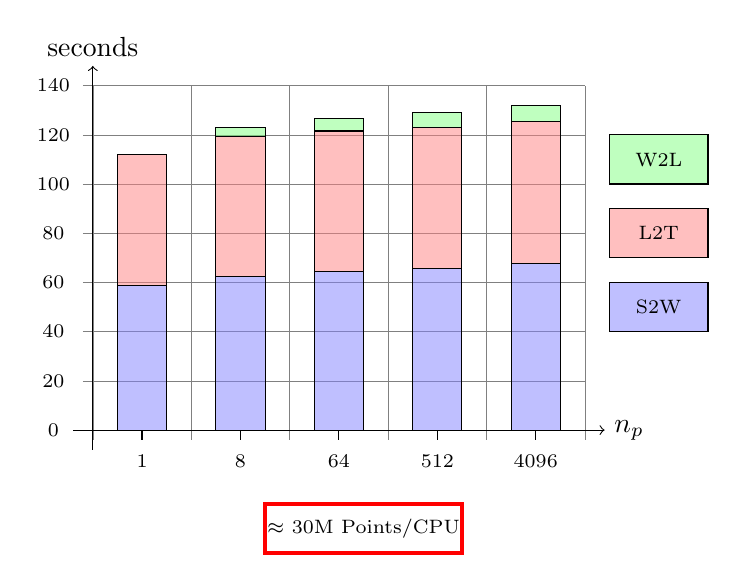
\begin{tikzpicture}[scale=1.25]

\draw[very thin, color=gray, xstep=1, ystep=0.5] (-0.1,-0.1) grid (5, 3.5);
\draw[->] (-0.2, 0) -- (5.2, 0) node[right] {$n_p$};
\draw[->] (0, -0.2) -- (0, 3.7) node[above] {seconds};

\newdimen\yscale

\yscale= 0.025 cm

\foreach \pos/\label in {0.5/1, 1.5/8, 2.5/64, 3.5/512, 4.5/4096} {
\draw (\pos,0) -- (\pos,-0.1) (\pos cm,-2.5ex) node [anchor=base,fill=white,inner sep=1pt]  {\scriptsize{\label}};
}

\foreach \label in {0, 20, ..., 140} {
 \draw (-0.4, \label\yscale) node {\scriptsize{\label}};
}

\draw[fill=blue!50, fill opacity=0.5] (4.5, 2.25) ++ (0.75, -1.25) rectangle +(1.0, 0.5);
\draw (4.5, 2.25) ++ (1.25, -1.0) node {\scriptsize{S2W}};

\draw[fill=red!50, fill opacity=0.5] (4.5, 1.75) ++ (0.75, 0.0) rectangle +(1.0, 0.5);
\draw (4.5, 1.75) ++ (1.25, 0.25) node {\scriptsize{L2T}};

\draw[fill=green!50, fill opacity=0.5] (4.5, 1.25) ++ (0.75, 1.25) rectangle +(1.0, 0.5);
\draw (4.5, 1.25) ++ (1.25, 1.5) node {\scriptsize{W2L}};

\draw[red, ultra thick] (1.75, -1.25) rectangle +(2.0, 0.5);
\draw (2.75, -1.0) node {\scriptsize{$\approx$ 30M Points/CPU}};

\newdimen\mypos
\newdimen\myoff

\foreach \pos/\vala/\valb/\valc/\vald/\vale/\valf in { 
0/58.75/53.36/0.0698/112.19/29.2M/$\frac{1}{16}$,
1/62.25/56.98/3.90/120.93/233.8M/$\frac{1}{64}$,
2/64.39/57.18/4.93/125.06/1.9B/$\frac{1}{256}$,
3/65.56/57.50/5.92/127.62/15.0B/$\frac{1}{1024}$,
4/67.53/57.75/6.59/131.65/119.7B/$\frac{1}{4096}$ } { 

\mypos=\pos cm
\advance \mypos by 0.5 cm

\advance \mypos by -0.25 cm

\myoff=0 cm

\draw[fill=blue!50, fill opacity=0.5] (\mypos, \myoff) rectangle +(0.5, \vala\yscale);
\advance \myoff by \vala\yscale

\draw[fill=red!50, fill opacity=0.5] (\mypos, \myoff) rectangle +(0.5, \valb\yscale);
\advance \myoff by \valb\yscale

\draw[fill=green!50, fill opacity=0.5] (\mypos, \myoff) rectangle +(0.5, \valc\yscale);

}

\end{tikzpicture}


	\end{center}
\caption{\label{f:isoUniform} Isogranular scalability for an uniform point distribution. For
 this experiment, we set $\epsilon = 10^{-6}$. The reported times for 
each component are the maximum values for that component across all the processors. The total wall-clock
time is reported in bold face.} \label{fig:uniform}
\end{figure}

{\em Example 2.} In this example, we consider a Gaussian random distribution of points in the unit cube. 
We present the weak scalability results in Figure \ref{fig:nonuniform}. 

\begin{figure}
	\begin{center}
	
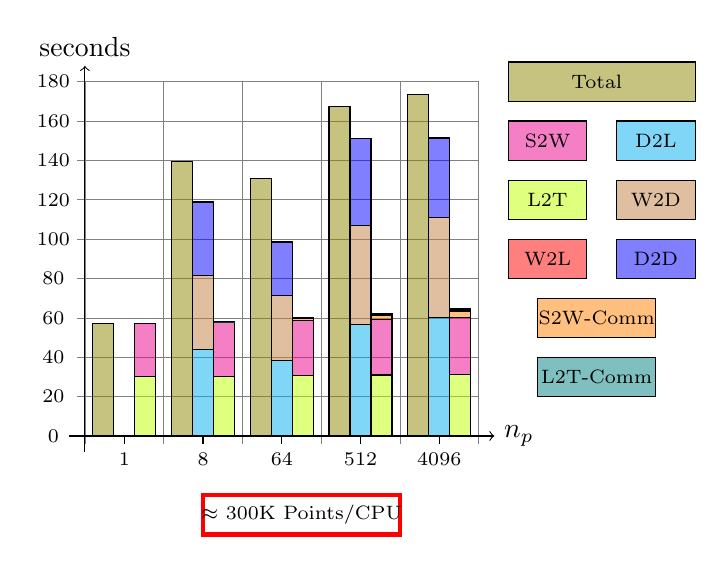
\begin{tikzpicture}[scale=1.0]

\draw[very thin, color=gray, xstep=1, ystep=0.5] (-0.1,-0.1) grid (5, 4.5);
\draw[->] (-0.2, 0) -- (5.2, 0) node[right] {$n_p$};
\draw[->] (0, -0.2) -- (0, 4.7) node[above] {seconds};

\newdimen\yscale

\yscale= 0.025 cm

\foreach \pos/\label in {0.5/1, 1.5/8, 2.5/64, 3.5/512, 4.5/4096} {
\draw (\pos,0) -- (\pos,-0.1) (\pos cm,-2.5ex) node [anchor=base,fill=white,inner sep=1pt]  {\scriptsize{\label}};
}

\foreach \label in {0, 20, ..., 180} {
 \draw (-0.4, \label\yscale) node {\scriptsize{\label}};
}


\draw[fill=olive, fill opacity=0.5] (5.375, 4.25) rectangle +(2.375, 0.5);
\draw (6.5, 4.5) node {\scriptsize{Total}};

\draw[fill=magenta, fill opacity=0.5] (5.375, 3.5) rectangle +(1.0, 0.5);
\draw (5.875, 3.75) node {\scriptsize{S2W}};

\draw[fill=lime, fill opacity=0.5] (5.375, 2.75) rectangle +(1.0, 0.5);
\draw (5.875, 3.0) node {\scriptsize{L2T}};

\draw[fill=red, fill opacity=0.5] (5.375, 2.0) rectangle +(1.0, 0.5);
\draw (5.875, 2.25) node {\scriptsize{W2L}};

\draw[fill=cyan, fill opacity=0.5] (6.75, 3.5) rectangle +(1.0, 0.5);
\draw (7.25, 3.75) node {\scriptsize{D2L}};

\draw[fill=brown, fill opacity=0.5] (6.75, 2.75) rectangle +(1.0, 0.5);
\draw (7.25, 3.0) node {\scriptsize{W2D}};

\draw[fill=blue, fill opacity=0.5] (6.75, 2.0) rectangle +(1.0, 0.5);
\draw (7.25, 2.25) node {\scriptsize{D2D}};

\draw[fill=orange, fill opacity=0.5] (5.75, 1.25) rectangle +(1.5, 0.5);
\draw (6.5, 1.5) node {\scriptsize{S2W-Comm}};

\draw[fill=teal, fill opacity=0.5] (5.75, 0.5) rectangle +(1.5, 0.5);
\draw (6.5, 0.75) node {\scriptsize{L2T-Comm}};

\draw[red, ultra thick] (1.5, -1.25) rectangle +(2.5, 0.5);
\draw (2.75, -1.0) node {\scriptsize{$\approx$ 300K Points/CPU}};


\newdimen\mypos
\newdimen\myoff

\foreach \pos/\vala/\valb/\valc/\vald/\vale/\valf/\valg/\valh/\vali/\valj/\valk/\vall/\valm in {
 0/0/0/0/30.07/27.18/0.0094/0.0045/0.014/57.28/827/0/283.7K/$\frac{1}{16}$,
 1/43.93/37.48/37.46/30.27/27.37/0.426/0.014/0.143/139.4/6666/6/2.3M/$\frac{1}{64}$,
 2/38.37/32.88/27.31/30.86/27.78/1.03/0.052/0.34/130.7/53929/126/18.5M/$\frac{1}{256}$,
 3/56.84/50.16/44.36/30.97/28.41/1.99/0.187/0.471/167.36/433226/880/148.9M/$\frac{1}{1024}$,
 4/60.18/50.65/40.56/31.08/29.24/3.18/0.567/0.924/173.42/3474244/7837/1.2B/$\frac{1}{4096}$
  } { 

\mypos=\pos cm
\advance \mypos by 0.5 cm

\advance \mypos by -0.4 cm
\myoff=0 cm

%Total

\draw[fill=olive, fill opacity=0.5] (\mypos, \myoff) rectangle +(0.266667, \vali\yscale);

%Direct

\advance \mypos by 0.266667 cm

\myoff=0 cm

\draw[fill=cyan, fill opacity=0.5] (\mypos, \myoff) rectangle +(0.266667, \vala\yscale);
\advance \myoff by \vala\yscale

\draw[fill=brown, fill opacity=0.5] (\mypos, \myoff) rectangle +(0.266667, \valb\yscale);
\advance \myoff by \valb\yscale

\draw[fill=blue, fill opacity=0.5] (\mypos, \myoff) rectangle +(0.266667, \valc\yscale);

%Expand

\advance \mypos by 0.266667 cm

\myoff=0 cm

\draw[fill=lime, fill opacity=0.5] (\mypos, \myoff) rectangle +(0.266667, \vald\yscale);
\advance \myoff by \vald\yscale

\draw[fill=magenta, fill opacity=0.5] (\mypos, \myoff) rectangle +(0.266667, \vale\yscale);
\advance \myoff by \vale\yscale

\draw[fill=orange, fill opacity=0.5] (\mypos, \myoff) rectangle +(0.266667, \valf\yscale);
\advance \myoff by \valf\yscale

\draw[fill=teal, fill opacity=0.5] (\mypos, \myoff) rectangle +(0.266667, \valg\yscale);
\advance \myoff by \valg\yscale

\draw[fill=red, fill opacity=0.5] (\mypos, \myoff) rectangle +(0.266667, \valh\yscale);

}

\end{tikzpicture}


	\end{center}
\caption{\label{f:isoGaussian} Isogranular scalability for a gaussian point distribution. For
 this experiment, we set $\epsilon = 10^{-3}$. The reported times for each component are the
 maximum values for that component across all the processors. The total wall-clock
time is reported in bold face.} \label{fig:nonuniform}
\end{figure}


%\section{Conclusions} \label{sc:conclusions}
%\input{conclusions.tex}

\newpage

%\appendix
%\input{appendix.tex}	

\bibliography{fgt}
\bibliographystyle{plain}
\end{document}


